\section{Durchführung}

Bei diesem Versuch wird der Brechungsindex von einem Prisma bestimmt. Dafür wird
ein Spektrometer verwendet, welches schematisch in Abbildung \ref{abb:2} dargestellt
ist.

\begin{figure}[H]
  \centering
  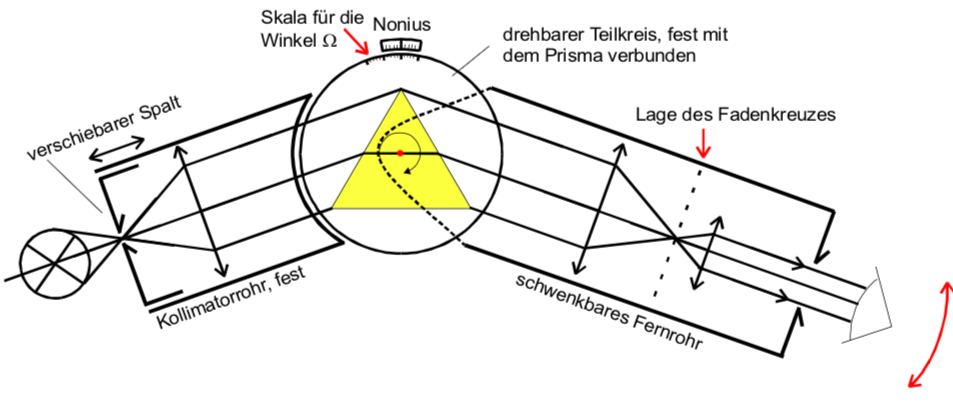
\includegraphics[width=\textwidth]{content/Spektrometer.png}
  \caption{Schematische Darstellung eines Spektrometers. \cite{1}}
  \label{abb:2}
\end{figure}

Zur Bestimmung des Brechungsindex $n$ dieses Prismas wird das Snelliussche Brechungsgesetz
aus Gleichung \ref{eq:2} umgeschrieben zu

\begin{equation}
  n = \frac{\sin(\frac{\eta + \varphi}{2})}{\sin(\frac{\varphi}{2})}.
  \label{eq:5}
\end{equation}

Die Bezeichnungen der Winkel gehen aus Abbildung \ref{abb:3} hervor.

\begin{figure}[H]
  \centering
  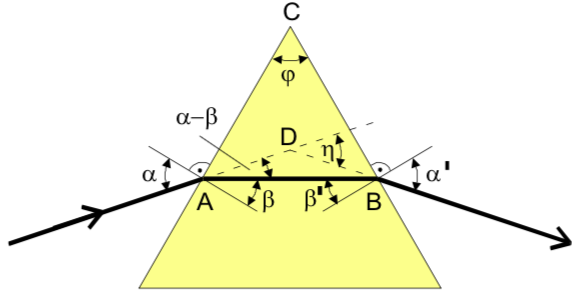
\includegraphics[width=\textwidth]{content/Prisma.png}
  \caption{Darstellung des Prismas mit der Bezeichnung der Winkel. \cite{1}}
  \label{abb:3}
\end{figure}

\subsection{\texorpdfstring{$\eta$} --Messung}

Bei dieser Messung wird das Prisma so gestellt, dass ein Teil des Lichtstrahls
reflektiert und ein Teil gebrochen wird. Der reflektierte Teil erscheint Weiß
in dem Fernrohr und der gebrochene Teil wird in seine Spektralfarben aufgespalten.
Das Prisma muss nun so ausgerichtet werden, dass der reflektierte Teil des Lichtes
auf der Spektralfarbe liegt, für welche $\eta$ bestimmt werden soll. Dabei wird die
Winkelstellung des Fernrohres $\Omega_l$ gemessen. Daraufhin wird diese Messung in
spiegelsymmetrischer Stellung des Prismas wiederholt und es wird wieder die Winkelstellung
des Fernrohrs $\Omega_r$ bestimmt. Damit lässt sich nun $\eta$ bestimmen

\begin{equation}
  \eta = 180 - (\Omega_r - \Omega_l).
  \label{eq:6}
\end{equation}

\subsection{\texorpdfstring{$\varphi$} --Messung}

Für Messung von $\varphi$ muss der Lichtstahl auf die Spitze fallen, wo sich der Winkel
$\varphi$ befindet. Dabei wird der Lichtstahl in zwei Richtungen reflektiert unter den
Winkeln $\varphi_r$ und $\varphi_l$. Mit diesen beiden Winkeln lässt sich nun $\varphi$ bestimmen

\begin{equation}
  \varphi = \frac{1}{2}(\varphi_r - \varphi_l)
  \label{eq:7}
\end{equation}
